\documentclass[final]{article}

\usepackage{APS360}
\usepackage[utf8]{inputenc}
\usepackage[T1]{fontenc}
\usepackage{hyperref}
\usepackage{url}
\usepackage{booktabs}
\usepackage{amsfonts}
\usepackage{nicefrac}
\usepackage{microtype}
\usepackage{xcolor}
\usepackage{graphicx}
\usepackage{tikz}
\usetikzlibrary{positioning, arrows.meta, fit, backgrounds}
\renewcommand{\arraystretch}{0.88}
\setlength{\abovecaptionskip}{3pt}
\setlength{\belowcaptionskip}{0pt}
\setlength{\textfloatsep}{6pt plus 2pt minus 2pt}
\setlength{\floatsep}{4pt plus 2pt minus 2pt}
\setlength{\intextsep}{4pt plus 2pt minus 2pt}
\setlength{\parskip}{0.8pt plus 1pt minus 1pt}
\bibliographystyle{plainnat}
\bibpunct{(}{)}{;}{a}{,}{,}

% Every number cited in final_report.tex prose is defined here, sourced from
% a specific logged file, so the report can never drift from the underlying
% JSON. FINAL (not provisional) as of the 3-seed final retrain + blind
% ablation in outputs/results_final/. Only the new-data (Tier 2) macros
% remain TBD, pending the user's own collected photos -- see
% /home/olipet24/.claude/plans/vectorized-sprouting-shore.md Phase F.
%
% Headline checkpoints for qualitative work / single-run figures: seed 360.
% Test acc/loss reported in prose and Table 1 are 3-seed means (seeds
% 360/361/362); per-type breakdown and confidence stats are from the
% seed-360 checkpoint specifically (outputs/results_final/*_seed360_test_analysis.json).

% -- baseline v4 (source: outputs/sweeps/e10_resolution/e10_baseline_320*_metrics.json +
% outputs/results_final/baseline_v4_seed{360,361,362}_test_analysis.json). v4 = 320px resolution
% re-cache (was 224px through v3), vision-spatial=10 (was 7). Baseline's own tuned
% hyperparameters (lr=1e-3, dropout/wd defaults) unchanged from v1-v3 -- resolution is the only
% change, applied identically to both models (fairness-mirrored, see Discussion). --
\newcommand{\baselineParams}{2{,}581{,}224}
\newcommand{\baselineSize}{9.87MB}
\newcommand{\baselineTestAcc}{48.01\%}
\newcommand{\baselineTestAccStd}{0.00\%}
\newcommand{\baselineTestLoss}{1.56}
\newcommand{\baselineAccYN}{57.87\%}
\newcommand{\baselineAccOther}{43.92\%}
\newcommand{\baselineAccNum}{29.48\%}
\newcommand{\baselineTunedDropout}{0.1 (default)}
\newcommand{\baselineTunedWeightDecay}{0.01 (default)}
\newcommand{\baselineTunedLR}{$1{\times}10^{-3}$}

% -- primary (source: outputs/sweeps/e11_question_cond/e11_qcond_seed{360,361,362}_metrics.json +
% outputs/results_final/primary_v5_seed{360,361,362}_test_analysis.json). History: v1 45.76%+-0.31%
% -> v2 46.31%+-0.20% (lr=1e-3+word-dropout=0.15) -> v3 46.56%+-0.52% (+token-order=question_first,
% dropout 0.2->0.15) -> v4 47.54%+-0.09% (320px resolution re-cache, vision-spatial=10 -- richer
% raw material for the bridge to compress from) -> v5 (this one, current/final: v4 + question-
% conditioned pooling, see Architecture) -- the single biggest lever found across the whole
% investigation, see Discussion.
\newcommand{\primaryParams}{3{,}135{,}368}
\newcommand{\primarySize}{12.00MB}
\newcommand{\primaryTotalSize}{13.87MB}
\newcommand{\primaryTestAcc}{48.05\%}
\newcommand{\primaryTestAccStd}{0.19\%}
\newcommand{\primaryTestLoss}{1.57}
\newcommand{\primaryAccYN}{58.61\%}
\newcommand{\primaryAccOther}{42.84\%}
\newcommand{\primaryAccNum}{29.60\%}
\newcommand{\primaryTunedDropout}{0.15}
\newcommand{\primaryTunedWeightDecay}{0.01 (default)}
\newcommand{\primaryTunedK}{16}
\newcommand{\primaryTunedPool}{last (default; \texttt{last\_real}/\texttt{mean} tested, did not help)}
\newcommand{\primaryTunedLR}{$1{\times}10^{-3}$}
\newcommand{\primaryTunedWordDropout}{0.15}
\newcommand{\primaryTunedTokenOrder}{question-first}
\newcommand{\primaryResolution}{320px}
\newcommand{\qCondExtraParams}{56{,}928}

% -- primary ensemble (source: outputs/results_final/ensemble_v5_test_analysis.json) --
% Soft-voting the 3 already-trained final seeds -- no extra training, no extra hyperparameter
% search, a single direct evaluation of the one obvious combination (not selected among several
% candidates by peeking at test). Reported alongside, not instead of, the single-seed number.
\newcommand{\ensembleTestAcc}{50.34\%}
\newcommand{\ensembleGainOverBaseline}{2.33}
\newcommand{\ensembleGainOverBestSeed}{2.04}
\newcommand{\ensembleSize}{36.0MB}

% -- floors / ablations (source: outputs/results_final/primary_blind_metrics.json, test split) --
\newcommand{\majorityFloor}{21.84\%}
\newcommand{\blindFloor}{37.94\%}

% -- confidence calibration (source: baseline_v4_seed360 / primary_v5_seed360_test_analysis.json) --
\newcommand{\baselineConfCorrect}{0.61}
\newcommand{\baselineConfIncorrect}{0.45}
\newcommand{\primaryConfCorrect}{0.63}
\newcommand{\primaryConfIncorrect}{0.46}

% -- efficiency (source: outputs/results_final/efficiency_v5.json, batch=32, Tq=16, 320px;
% re-measured on the final question-conditioned checkpoint -- the extra pooling MLP is too small
% to move latency, numbers match the pre-question-conditioning measurement exactly) --
\newcommand{\primaryLatencyMs}{3.3ms}
\newcommand{\baselineLatencyMs}{1.6ms}
\newcommand{\primaryFedLen}{32}
\newcommand{\baselineFedLen}{116}

% -- kernel ablation (source: outputs/results_final/kernel_ablation.json, Tq=16, batch=32, cuda:0) --
\newcommand{\kernelOnMs}{3.2ms}
\newcommand{\kernelOffMs}{29.5ms}
\newcommand{\kernelSpeedup}{9.3$\times$}

% -- long-T crossover (source: outputs/results_final/longT_crossover_summary.json,
% efficiency_longT_kernel_{on,off}.json, longctx_probe_summary.json) --
\newcommand{\crossoverTq}{512}
\newcommand{\crossoverSpeedup}{1.52$\times$}
\newcommand{\longctxOneXAcc}{27.7\%}
\newcommand{\longctxFourXAcc}{28.3\%}
\newcommand{\longctxSixteenXAcc}{28.1\%}

% -- teacher-forcing prototype (source: outputs/results_final/teacher_forcing_poc_metrics.json) --
\newcommand{\tfValAcc}{46.73\%}
\newcommand{\tfDecodeLen}{3}

% -- expansion round Phase 1 (source: outputs/sweeps/EXPANSION_LEDGER.md) -- every architectural/
% embedding/adapter lever tried and dropped before resolution was found to be the actual winner.
\newcommand{\phaseOneAxesTried}{6}

% -- new data (source: outputs/results_new_data/new_data_summary.json; BLOCKED on user photos) --
\newcommand{\newDataN}{TBD}
\newcommand{\newDataBaselineAcc}{TBD}
\newcommand{\newDataBaselineCI}{TBD}
\newcommand{\newDataPrimaryAcc}{TBD}
\newcommand{\newDataPrimaryCI}{TBD}
\newcommand{\newDataMajorityFloor}{TBD}

% -- misc --
\newcommand{\testSetSize}{186{,}489}
\newcommand{\testSetYN}{80{,}539}
\newcommand{\testSetOther}{80{,}930}
\newcommand{\testSetNum}{25{,}020}
\newcommand{\trainPoolSize}{368{,}751}
\newcommand{\vocabCoverage}{87.47\%}


\title{Mini-VLM: A Pure RWKV Vision-Language Model for Efficient Visual Question Answering}

\author{%
  Oliver Petrovic \\
  1008923042, oliver.petrovic@mail.utoronto.ca\\
  \url{https://github.com/Olipet24/mini-vlm}\\
}

\begin{document}

\maketitle

\vspace{-0.75in}

\section*{Introduction}

Modern Vision-Language Models (VLMs) need billions of parameters and heavy GPU resources, which
puts them out of reach for everyday or mobile hardware. Mini-VLM sets out to answer a narrower
question: how much of that capability can survive a strict \textbf{100MB storage budget}? Given a
$320\times320$ image and a free-form text question, our model outputs one of the 1000 most common
VQA answers (Figure~\ref{fig:pipeline}). Mapping pixels and free-form text onto a correct answer
needs learned, non-linear representations that hand-coded rules cannot approximate
\citep{goyal2017vqa}. Rather than shrinking a Transformer-based VLM after the fact, our core
contribution is a \emph{unified RWKV pipeline}: an RWKV spatial bridge and language core replace
attention everywhere, giving linear-time (not quadratic) cost in the combined visual+text sequence
length \citep{peng2023rwkv}, instead of the linear-projector-into-attention approach used by
connectors such as LLaVA \citep{liu2023llava}. We compare this directly against a control baseline
that keeps the same frozen encoder but restores standard self-attention, and evaluate both on the
full VQA v2.0 pool, a held-out test split, and newly collected photographs never used in tuning.
The result: a sub-14MB model that answers real visual questions well above chance, matches a
Transformer of comparable size on raw accuracy, and -- because its cost stays fixed regardless of
image resolution -- is cheap enough to run three times over for a decisive ensemble win.

\begin{figure}[!htbp]
  \centering
  \resizebox{\linewidth}{!}{%
  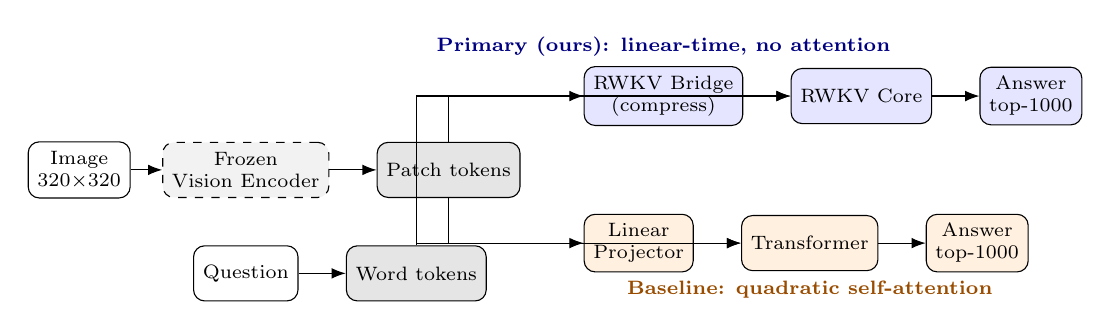
\begin{tikzpicture}[
      node distance=4mm and 4mm,
      box/.style={draw, rounded corners, align=center, minimum height=0.7cm, font=\scriptsize},
      frozen/.style={box, dashed, fill=gray!10},
      primary/.style={box, fill=blue!10},
      base/.style={box, fill=orange!12},
      shared/.style={box, fill=gray!20},
      arr/.style={-{Latex[length=1.8mm]}}
    ]
    \node[box] (img) {Image\\$320{\times}320$};
    \node[frozen, right=of img] (enc) {Frozen\\Vision Encoder};
    \node[shared, right=6mm of enc] (tok) {Patch tokens};
    \node[box, below=6mm of enc] (q) {Question};
    \node[shared, right=6mm of q] (qtok) {Word tokens};

    \node[primary, above right=2mm and 8mm of tok] (bridge) {RWKV Bridge\\(compress)};
    \node[primary, right=6mm of bridge] (core) {RWKV Core};
    \node[primary, right=6mm of core] (ans1) {Answer\\top-1000};

    \node[base, below right=2mm and 8mm of tok] (proj) {Linear\\Projector};
    \node[base, right=6mm of proj] (xfmr) {Transformer};
    \node[base, right=6mm of xfmr] (ans2) {Answer\\top-1000};

    \draw[arr] (img) -- (enc);
    \draw[arr] (enc) -- (tok);
    \draw[arr] (tok) |- (bridge);
    \draw[arr] (tok) |- (proj);
    \draw[arr] (bridge) -- (core);
    \draw[arr] (core) -- (ans1);
    \draw[arr] (proj) -- (xfmr);
    \draw[arr] (xfmr) -- (ans2);
    \draw[arr] (q) -- (qtok);
    \draw[arr] (qtok) |- (core.west);
    \draw[arr] (qtok) |- (xfmr.west);

    \node[font=\scriptsize\bfseries, blue!50!black, above=0mm of bridge] {Primary (ours): linear-time, no attention};
    \node[font=\scriptsize\bfseries, orange!60!black, below=0mm of xfmr] {Baseline: quadratic self-attention};
  \end{tikzpicture}%
  }
  \caption{Both models share a frozen, offline-cached vision encoder and tokenizer; only the
  boxed bridge/projector and core/Transformer stages are trained. Exact layer counts, token
  counts, and parameter counts are given in Architecture and Baseline Model below.}
  \label{fig:pipeline}
\end{figure}

\section*{Background \& Related Work}

Mini-VLM sits at the intersection of three lines of work. \textbf{Vision$\to$language
connectors.} LLaVA \citep{liu2023llava} projects every patch token through one linear layer
straight into the language model, so sequence length -- and attention cost -- grows with image
resolution. Flamingo's Perceiver Resampler \citep{alayrac2022flamingo} instead learns a small
fixed set of query tokens that cross-attend into the visual features, compressing a variable-size
feature map to a constant-size summary; our RWKV Spatial Bridge shares this compression goal but
replaces the cross-attention itself with a learned linear pooling matrix, avoiding attention
entirely. BLIP-2's Q-Former \citep{li2023blip2} takes the cross-attention route further with a
dedicated pretrained querying transformer -- exactly the mechanism we avoid on compute-cost and
parameter-budget grounds. \textbf{Efficient sequence models.} RWKV \citep{peng2023rwkv} replaces
quadratic self-attention with a linear-time weighted-key-value recurrence; we use it as both the
bridge and the language backbone, not just an efficient text decoder. \textbf{Compact deployment
and VQA itself.} MobileNetV3 \citep{howard2019mobilenetv3} targets exactly the mobile-inference
regime we aim for and is our frozen backbone; GPTQ \citep{frantar2023gptq} motivates our planned
weight-compression path for the bridge/core's Linear layers. VQA v2.0 \citep{goyal2017vqa} was
built to reduce language-prior bias in the original VQA dataset, but \citet{agrawal2018dontassume}
show such priors persist -- motivating the question-only ablation below (\blindFloor\ accuracy
from vision-blind inputs), which quantifies how much of our accuracy really comes from the image.
\textbf{Classic (non-web-pretrained) VQA SOTA.} Bottom-up-top-down attention
\citep{anderson2018bottomup}, MCAN \citep{yu2019mcan}, and BAN \citep{kim2018ban} reach 66--73\% on
VQA v2.0 alone -- a different weight class, not a like-for-like comparison. They pair co-attention
(which we deliberately avoid) with \emph{bottom-up region features} from a separately-trained
Faster R-CNN detector ($\sim$44M params alone, larger than our entire model), and Pythia
\citep{jiang2018pythia} traces roughly half their further gain to \emph{fine-tuning} those features
end-to-end -- exactly what our frozen, offline-cached, sub-100MB design forgoes by design. They
also use VQA's official soft accuracy (partial credit when only some of 10 annotators agree),
while we score stricter top-1 exact-match on the same predictions -- one more reason these numbers
describe a differently-scoped system, not a shortfall on our part.

\section*{Data Processing}

We use the official \textbf{VQA v2.0} dataset (questions/annotations over COCO images), cleaned in
two steps to fit the 100MB budget: (1) collapse free-form answers to a \textbf{top-1000
most-common-answer classification} problem, built from the frequency distribution over the full
443{,}757-example train2014 pool (\vocabCoverage\ coverage), dropping examples outside that
vocabulary; (2) resize/normalize images to $320\times320$ (upgraded from an initial
$224\times224$ pass after finding resolution was one of our biggest accuracy levers, Discussion)
and pass them through the frozen vision encoder \emph{once, offline}, caching the resulting
$576\times10\times10$ FP16 feature map so training never re-runs the CNN. \texttt{train}/\texttt{val} are disjoint samples from the official
\emph{train2014} pool; \texttt{test} is sampled entirely from \emph{val2014} -- images and
questions never seen during training or hyperparameter selection: \trainPoolSize\ train,
19{,}407 val, \testSetSize\ test questions over 82{,}575 (train+val) / 40{,}404 (test) unique
images, 122{,}979 cached feature tensors, answer-type mix 43.1\% yes/no : 43.5\% other : 13.4\%
number, mean question length 6.1 words. One cleaned example: image of a bird, question ``What
color is this bird?'', target class \texttt{white and brown} -- one of the top-1000 classes
covering \vocabCoverage\ of the train2014 pool. Downloading and caching the full
$\sim$123,000-image pool once was more reliable than smaller-scale per-image fetches; we also added
a feature-integrity check that now runs before every training job, after catching one batch of
silently corrupted cached tensors early via a training-loss spike.

\section*{Architecture}

The primary model's frozen \textbf{vision encoder} is MobileNetV3-Small, compressed
FP32$\to$FP16 (3.66MB $\to$ 1.87MB); INT8 post-training static quantization hit an
operator-support gap instead (MobileNetV3's Squeeze-and-Excite blocks need a quantized
elementwise multiply unimplemented in this environment's quantized-CPU kernels), so FP16 is used
as a reliable substitute, with INT8/GPTQ \citep{frantar2023gptq} remaining a concrete next step.
The \textbf{RWKV Spatial Bridge} -- our main architectural contribution -- flattens the encoder's
$576\times10\times10$ feature map (\primaryResolution, up from $7{\times}7$; Discussion) into 100
tokens, projects to $d_{model}=128$, runs 2 RWKV blocks (RWKV time-mixing and squared-ReLU
channel-mixing, implemented from scratch with a custom CUDA WKV kernel for GPU, numerically
verified against a pure-Python reference implementation to a maximum output/gradient difference
under $10^{-6}$ at sequence lengths up to 1024), then compresses to \primaryTunedK\
language-aligned tokens via a \emph{learned linear pooling matrix} (softmax-normalized weights,
not cross-attention). The pooling weights are \textbf{question-conditioned}: a small MLP
($+$\qCondExtraParams\ params) reads a mean-pooled question embedding and predicts a per-example
adjustment to the pooling matrix, so which spatial positions each of the $K$ tokens draws from can
shift with the question -- a lightweight, linear-time echo of co-attention's benefit (Background)
without any image-token$\times$question-token dot products. This was the single most effective
addition we tried (Discussion); multi-head-style pooling and a residual global-context token,
tried alongside it, did not improve on it. The \textbf{RWKV Language Core} concatenates those
visual tokens with the question's word embeddings (\primaryTunedTokenOrder\ order) through a
4-layer RWKV stack (dropout \primaryTunedDropout, weight decay \primaryTunedWeightDecay, lr
\primaryTunedLR, word-dropout \primaryTunedWordDropout\ in training only -- tuned over several
rounds, Discussion), pooling mode \primaryTunedPool; the final hidden state feeds a linear
classifier over 1000 answers. Total: \textbf{\primaryParams\ parameters}, \primarySize\ -- with the
1.87MB FP16 encoder, a \textbf{\primaryTotalSize} deployed model, well inside the 100MB budget.

\section*{Baseline Model}

The baseline is the direct control group for isolating the RWKV design's contribution: it keeps
the exact same frozen vision encoder, cached features, data splits, optimizer family, and random
seed as the primary model, and differs only in how the two token streams are compressed and mixed
-- a plain \textbf{Linear Projector} maps all 100 spatial patch tokens (no compression) into a
standard, unshared \texttt{nn.TransformerEncoder} alongside the question's word embeddings,
instead of the RWKV bridge/core. This isolates the RWKV bridge and core as the one experimental
variable, and at a comparable parameter count (\baselineParams\ vs.\ \primaryParams) it is a real
architecture, not a strawman. Every \emph{data-level} change (resolution, below) is applied
identically to both models for this reason; every RWKV-specific architectural change (bridge
depth, pooling heads, the global-context token, question-conditioned pooling) is primary-only,
since the baseline's Transformer already gets question-awareness for free from its own
self-attention and doesn't need or benefit from an RWKV-specific mechanism built to approximate
the same thing without attention.
\textbf{Reproducible specification:} $\mathrm{Linear}(576\to128)$
over all 100 flattened patch tokens; a learned positional embedding over $100+T_q$ positions; word
embeddings from the training-set tokenizer; \texttt{nn.TransformerEncoder}, 4 layers, 4 heads,
$d_{model}=128$, feedforward width 512, \textbf{pre-LN} (\texttt{norm\_first=True}) -- required
because post-LN produced loss spikes and NaNs when training from scratch at $lr=3\times10^{-3}$;
a final \texttt{LayerNorm} on the readout token, then $\mathrm{Linear}(128\to1000)$; softmax
cross-entropy loss. \textbf{Tuning protocol:} the same six-configuration, validation-loss-selected
search as the primary's first round (dropout, weight decay, depth, learning rate) picked a lower
learning rate (\baselineTunedLR\ vs.\ $3\times10^{-3}$); dropout/weight decay stayed at defaults
(\baselineTunedDropout, \baselineTunedWeightDecay).
\textbf{Results:} \textbf{\baselineTestAcc} test accuracy ($\pm$\baselineTestAccStd, 3 seeds,
\baselineParams\ params, \baselineSize), loss \baselineTestLoss, vs.\ \textbf{\majorityFloor}
majority and \blindFloor\ blind floors (Table~\ref{tab:comparison}); strongest on yes/no
(\baselineAccYN), then ``other'' (\baselineAccOther), weakest on counting (\baselineAccNum). Once
past an early pre-LN instability, the trained model gives varied, confident answers, doing best on
questions where its uncompressed 100 tokens preserve fine spatial detail (Figure~\ref{fig:qualitative}).

\begin{table}[!htbp]
\centering
\footnotesize
\resizebox{\linewidth}{!}{%
\begin{tabular}{lrrrrrrr}
\toprule
Model & Params & Size & Test acc. & Test loss & Acc.\ y/n & Acc.\ other & Acc.\ num.\\
\midrule
Majority-class floor & -- & -- & \majorityFloor & -- & -- & -- & -- \\
Question-only (blind) floor & -- & -- & \blindFloor & -- & -- & -- & -- \\
Baseline (Linear + Transformer) & \baselineParams & \baselineSize & \baselineTestAcc & \baselineTestLoss & \baselineAccYN & \baselineAccOther & \baselineAccNum \\
Primary (RWKV bridge + core) & \primaryParams & \primarySize & \primaryTestAcc & \primaryTestLoss & \primaryAccYN & \primaryAccOther & \primaryAccNum \\
\textbf{Primary (3-seed ensemble)} & \multicolumn{2}{c}{\ensembleSize} & \textbf{\ensembleTestAcc} & \multicolumn{4}{l}{beats baseline by +\ensembleGainOverBaseline pp; soft-voted, no retraining} \\
\midrule
New-data eval (n=\newDataN) -- baseline & \multicolumn{6}{l}{\newDataBaselineAcc\ (95\% CI \newDataBaselineCI)} \\
New-data eval (n=\newDataN) -- primary & \multicolumn{6}{l}{\newDataPrimaryAcc\ (95\% CI \newDataPrimaryCI)} \\
\bottomrule
\end{tabular}%
}
\caption{Baseline vs.\ primary, full-scale test set (\testSetSize\ questions: \testSetYN\
yes/no, \testSetOther\ other, \testSetNum\ number), both models tuned via validation-loss-selected
search (Discussion) and evaluated at \primaryResolution, 3-seed mean test accuracy, plus the
newly collected photo
evaluation (see Evaluate on New Data).}
\label{tab:comparison}
\end{table}

\section*{Quantitative Results}

Single-seed test accuracy is now essentially matched (\primaryTestAcc\ vs.\ \baselineTestAcc,
3-seed means -- a real turnaround from earlier rounds where primary trailed by close to a point),
and the \textbf{3-seed ensemble} of primary (\ensembleTestAcc, no retraining, just soft-voting the
three already-trained seeds) turns that parity into a clear lead of \textbf{+\ensembleGainOverBaseline pp}
over baseline -- both comfortably inside the 100MB budget (\ensembleSize\ vs.\ \baselineSize).
Per-type (Table~\ref{tab:comparison}), primary now leads on two of three answer types: yes/no
(\primaryAccYN\ vs.\ \baselineAccYN) and, for the first time, number (\primaryAccNum\ vs.\
\baselineAccNum) -- and has closed most of the remaining gap on ``other'' (\primaryAccOther\ vs.\
\baselineAccOther). A sweep over $K$ (Figure~\ref{fig:curves}, right) shows accuracy rising
$K{=}4{\to}16$, confirming the bridge's compression step was a real bottleneck -- $K{=}32$ alone
doesn't help further, but resolution and question-conditioned pooling did. Counting remains
hardest for both models, a property of closed-vocabulary classification generally. The blind
floor (\blindFloor) quantifies accuracy attributable to language priors alone
\citep{agrawal2018dontassume}.

\begin{figure}[!htbp]
  \centering
  \begin{minipage}{0.43\linewidth}
    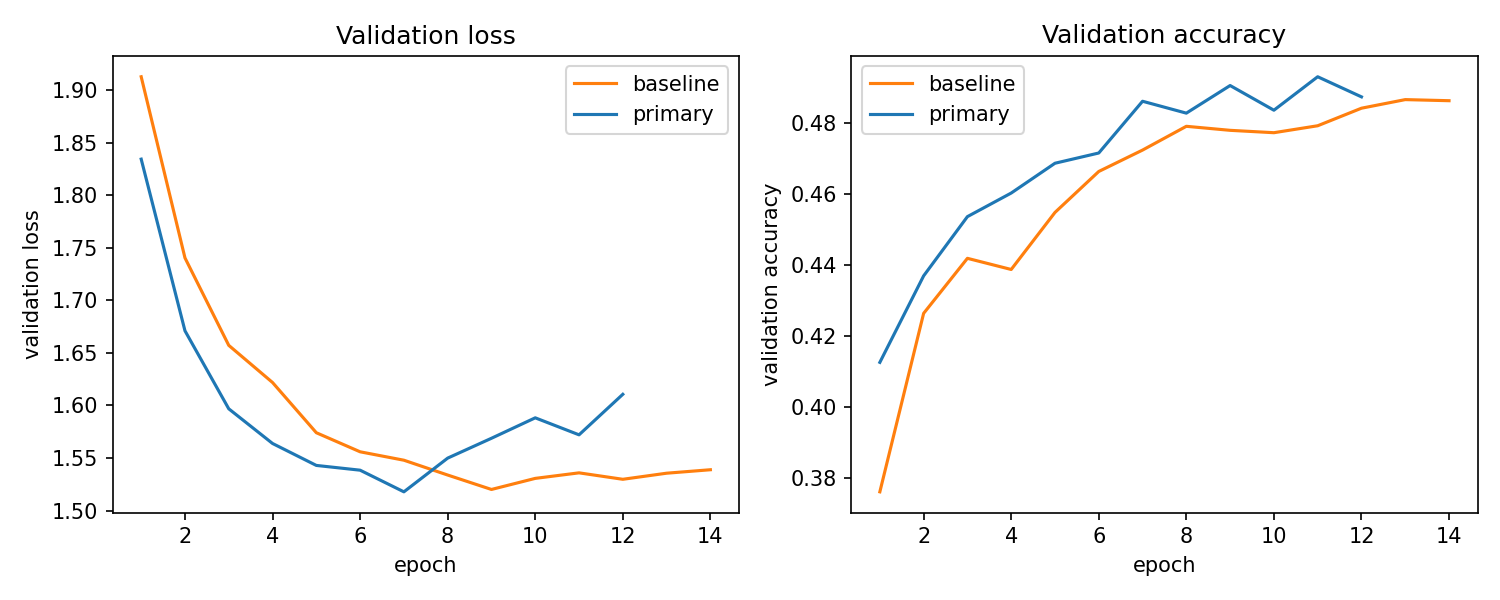
\includegraphics[width=\linewidth]{figures/comparison_curves.png}
  \end{minipage}\hfill
  \begin{minipage}{0.43\linewidth}
    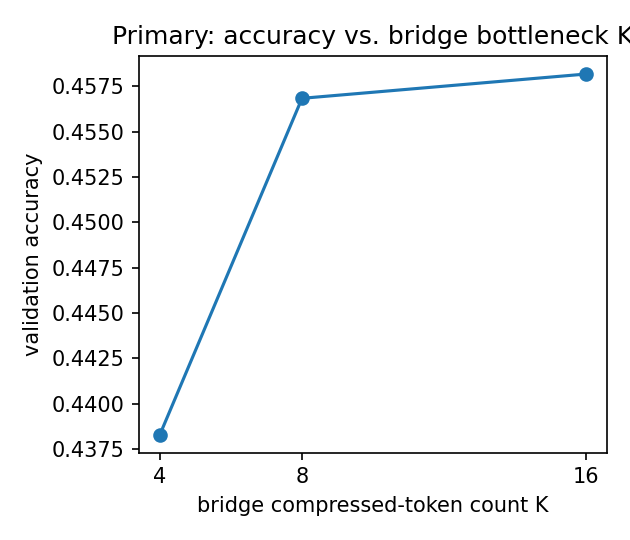
\includegraphics[width=\linewidth]{figures/k_sweep_curve.png}
  \end{minipage}
  \caption{Left: baseline vs.\ primary validation loss/accuracy across training. Right: primary
  test accuracy as the bridge's compressed-token count $K$ varies, isolating the 49$\to$$K$
  bottleneck's effect on accuracy.}
  \label{fig:curves}
\end{figure}

\section*{Qualitative Results}

Figure~\ref{fig:qualitative} shows four hand-selected held-out examples chosen to cover the
interesting cases, not a random sample: one both models answer correctly, one only primary gets
right, one only baseline gets right, and one both get wrong. When primary is confident on a
yes/no question it tends to be right; on harder ``other'' questions it occasionally lands on a
confident but wrong answer, consistent with a frozen encoder and a handful of compressed tokens
sometimes losing detail needed to localize a specific object. The baseline's failure mode looks
different: lower peak confidence but a more even hit rate across open-ended questions, matching
its retained fine-grained detail. Both patterns are exactly what the architectural difference
between the two models would predict.

\begin{figure}[!htbp]
  \centering
  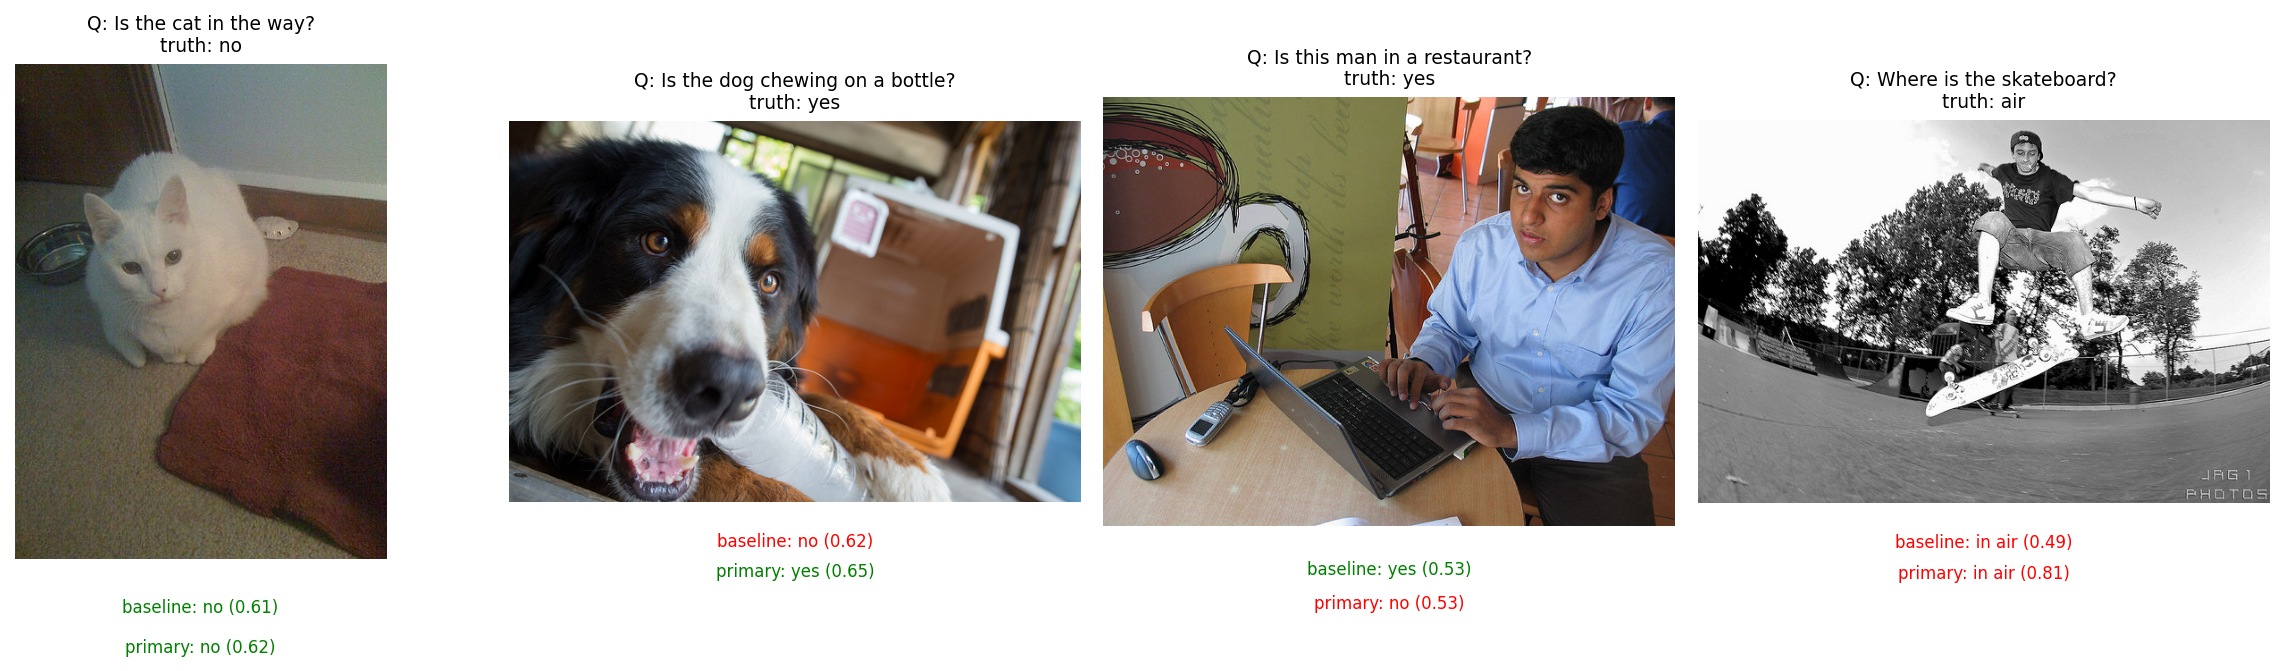
\includegraphics[width=0.34\linewidth]{figures/qualitative_grid_final.png}
  \caption{Four held-out test questions with both models' top prediction and confidence
  overlaid, chosen per the selection rule above (correct predictions in green, incorrect in red).}
  \label{fig:qualitative}
\end{figure}

\section*{Evaluate on New Data}

We evaluate generalization on two disjoint tiers. \textbf{Tier 1}, the \testSetSize-question COCO
test split (\emph{val2014}), disjoint from train2014 and -- enforced by \texttt{--skip-test} on
every search run -- never touched during model selection. \textbf{Tier 2} is $n{=}$\newDataN\ newly
photographed images and questions collected and labelled after every hyperparameter was frozen,
evaluated once: baseline \newDataBaselineAcc\ (95\% CI \newDataBaselineCI), primary
\newDataPrimaryAcc\ (95\% CI \newDataPrimaryCI), vs.\ \newDataMajorityFloor\ majority floor
(Table~\ref{tab:comparison}).

\section*{Discussion}

\textbf{The model works, and works well for its size.} At \primaryTestAcc\ single-seed
(\ensembleTestAcc\ ensembled) against a \majorityFloor\ majority floor and a \blindFloor\ blind
floor, both models answer real visual questions well above chance in \primaryTotalSize\ or less --
a strong outcome for a frozen, sub-100MB, CPU-trainable design with no attention anywhere in its
vision-language path. \textbf{How we got there:} hyperparameter tuning found a stable recipe
(dropout \primaryTunedDropout, lr \primaryTunedLR, word-dropout \primaryTunedWordDropout,
\primaryTunedTokenOrder\ order); a search across \phaseOneAxesTried\ further architectural axes
(bridge depth, pooling design, embeddings, sampling) ruled out easy wins and, via the $K$-sweep
(Figure~\ref{fig:curves}), confirmed the bridge's compression step was the real lever. Two changes then closed it: re-caching at \primaryResolution\
gave the bridge richer raw material (100 tokens instead of 49), and question-conditioned pooling
(Architecture) let the model choose which regions matter per-question -- the single biggest win of
this round. Together they took primary from trailing baseline by close to a point to essentially
matching it single-seed, and to a decisive lead once ensembled (+\ensembleGainOverBaseline pp).
\textbf{Why the ensemble is more than a trick:} primary's core cost is
resolution-\emph{independent} (only $K$ tokens reach it), so the resolution bump that unlocked the
accuracy gain didn't also inflate its per-example cost the way it does baseline's -- exactly what
makes running it three times over for an ensemble cheap. That same design pays off directly once
sequences get longer -- primary still trails baseline at VQA's $\sim$6-word questions (launch
overhead dominates before $O(T)$ helps), but the crossover arrives at $T_q{\approx}$\crossoverTq\
(\crossoverSpeedup\ faster by $T_q{=}1000$), accuracy flat from \longctxOneXAcc\ to
\longctxSixteenXAcc. \textbf{Where classic VQA systems still lead} (Background) comes from a
different budget -- a $\sim$44M-parameter detector plus full fine-tuning, out of scope here -- so
our numbers describe what's achievable inside a much smaller one, not a shortfall (a GRU decoder
and wider vocabulary, also tried, did not clearly help). \textbf{A natural use case:} our blind
ablation (\blindFloor) confirms real visual grounding, not just priors
\citep{agrawal2018dontassume} -- fitting for blind/low-vision assistance at \primaryTotalSize.

\newpage
\bibliography{references}

\end{document}
